\documentclass[a4paper,11pt]{article}
\usepackage[T1]{fontenc}
\usepackage[utf8]{inputenc}
\usepackage{lmodern}
\usepackage{amsmath}
\usepackage{amsfonts}
\usepackage{amssymb}
\usepackage{amsthm}
\usepackage{graphicx}
\usepackage{url}
\usepackage{listings}
\usepackage{hyperref}
\usepackage{parskip}
\usepackage{todonotes}
\usepackage{caption}
\usepackage{subcaption}
\usepackage{float}

%%%%%%%%%%%%%%%%%%%
% For Gantt chart %
%%%%%%%%%%%%%%%%%%%
\usepackage{pgfgantt}

%%%%%%%%%%%%%%%%%%%%%
% For float barrier %
%%%%%%%%%%%%%%%%%%%%%
\usepackage{placeins}

%%%%%%%%%%%%%%%%%%%%
% For bibliography %
%%%%%%%%%%%%%%%%%%%%
\usepackage[citestyle=numeric,style=numeric,sorting=none, maxnames=2, giveninits=true, backend=biber]{biblatex}
\addbibresource{bibliography.bib}

\title{\textbf{Thesis Specification} \\ Automatic Assessment of Focus Quality in Microscopy Images}
\author{Hannes F. Kuchelmeister}
\date{\today}

\begin{document}

\begin{titlepage}
\maketitle

%\tableofcontents
%\newpage

%\begin{abstract}
%\end{abstract}

\thispagestyle{empty}
\newpage
\end{titlepage}

\section{Background}

\todo[inline]{Here you describe in what context your thesis is to be done. What prerequisites are valid, what is the goal of the project from the supervisors point of view, what is available and has been done before, under what circumstances should the work be done.}

Neglected Tropical Diseases (NTDs) \cite{worldhealthorganization2021neglected} are a set of diseases mainly present in tropical and subtropical regions of the world, affecting more than a billion people across the globe. Almost exclusively affecting poor regions, many of the diseases can be prevented or even completely eradicated given proper access to existing technologies and tools. However, affected populations are often of low socio-economic status and of low priority in public health efforts. One particular class of NTDs are Soil-Transmitted Helminths (STHs) \cite{worldhealthorganization2020soiltransmitted}: Ascaris, whipworm and hookworm. These are intestinal, parasitic worms transmitted through contaminated soil. Each type of STH is estimated to affect between 500 million to 1 billion people on a global scale. As intestinal worms, the eggs of STHs are spread through the faeces of the infected. 

Part of the effort to detect STH infections has been to look for parasite eggs under a microscope. Specifically, stool samples are examined, where egg counts determine infection status. However, due to long training time of staff and high turnover rate, an automated solution could prove to be much more efficient. Such a solution is under development at Etteplan Sweden.

Etteplan’s solution, an automated microscope, scans glass slides with samples prepared according to the Kato-Katz technique \cite{worldhealthorganization1991basic}, in a whole slide imaging fashion \cite{hanna2019whole}. A slide is partitioned into a grid, where each grid cell corresponds to the camera’s field of view in that position. The sample has the obvious spatial extension tangential to the glass plane, but also a non-negligible spatial distribution along the optical axis, compared to the camera's depth of field. Hence, the camera takes multiple images of the grid cell, varying the focal plane, to capture as much of the information of the sample in each grid cell, a process called z-stacking. The result is multiple images of each grid cell, with different regions of the image being in focus for different positions of the focal plane. A sample can be seen in \autoref{fig:focusComparison}.

\begin{figure}
    \begin{subfigure}[t]{0.3\textwidth}
        \centering
        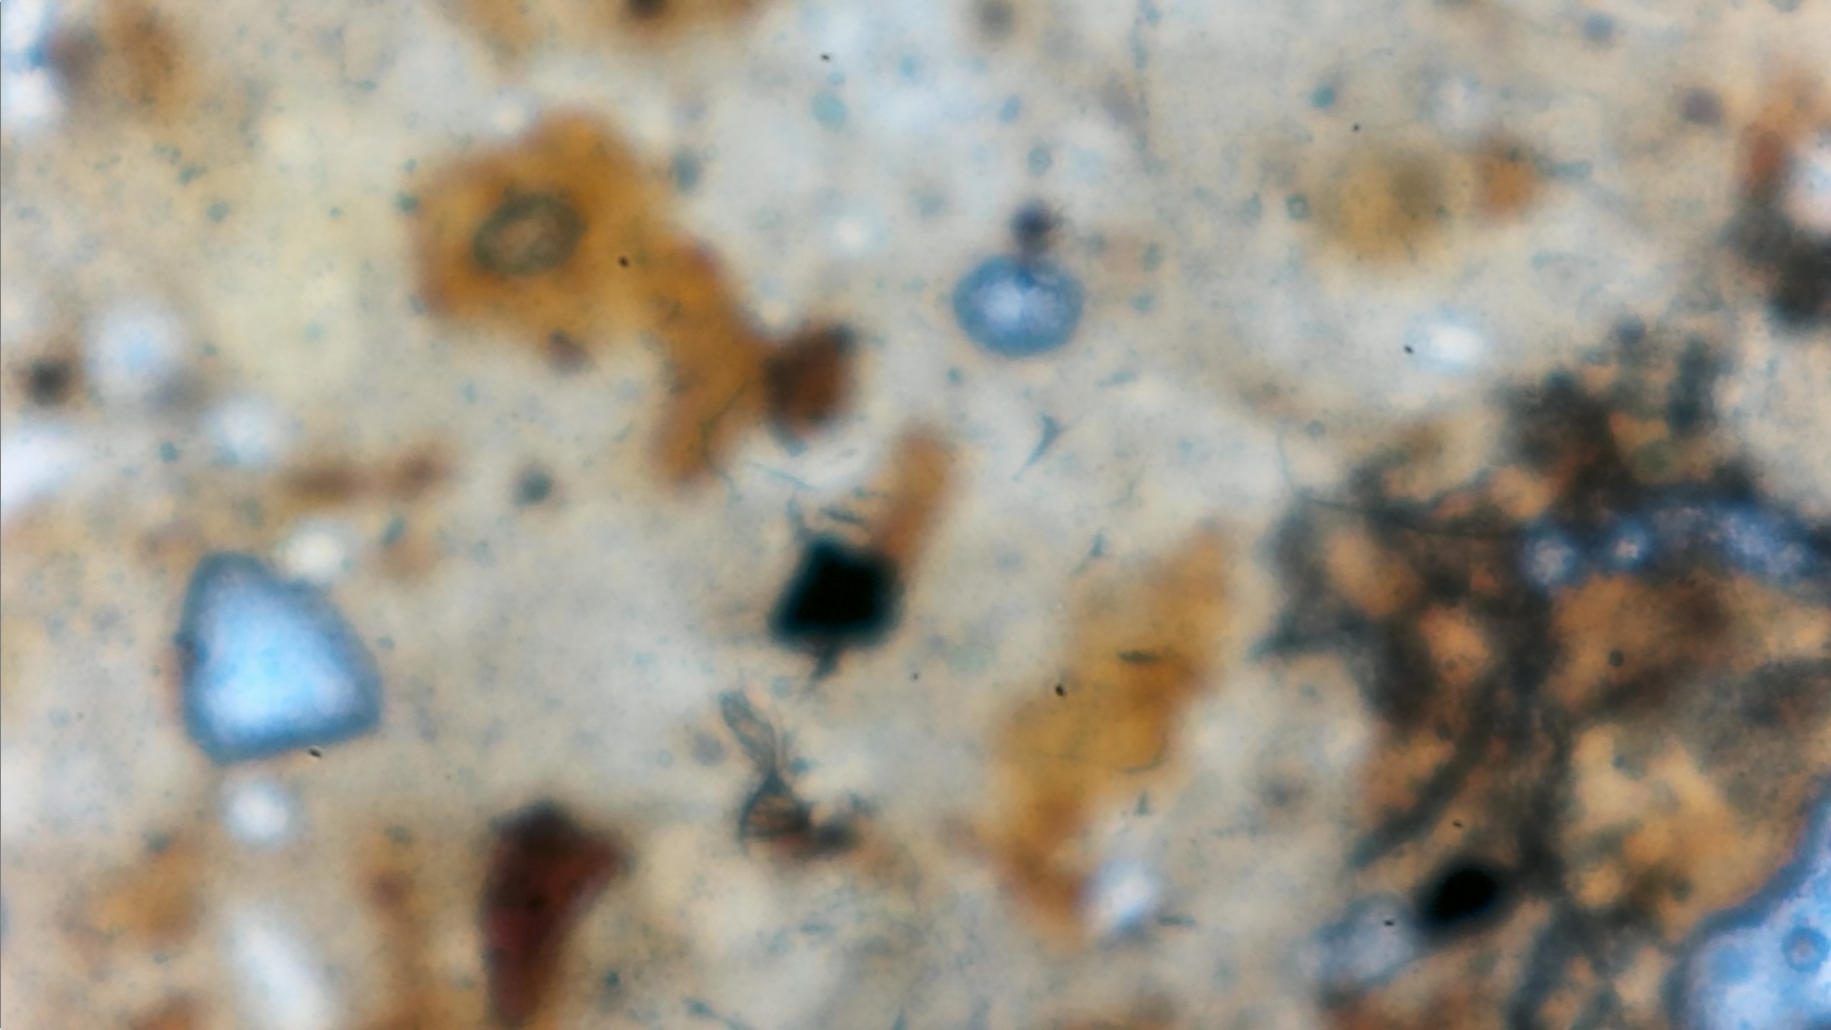
\includegraphics[width=\textwidth]{./img/out_of_focus_hither.png}
        \caption{Out-of-focus image with focal plane hither to sample.}
        \label{fig:focusHither}
    \end{subfigure}
    \hfill
    \begin{subfigure}[t]{0.3\textwidth}
        \centering
        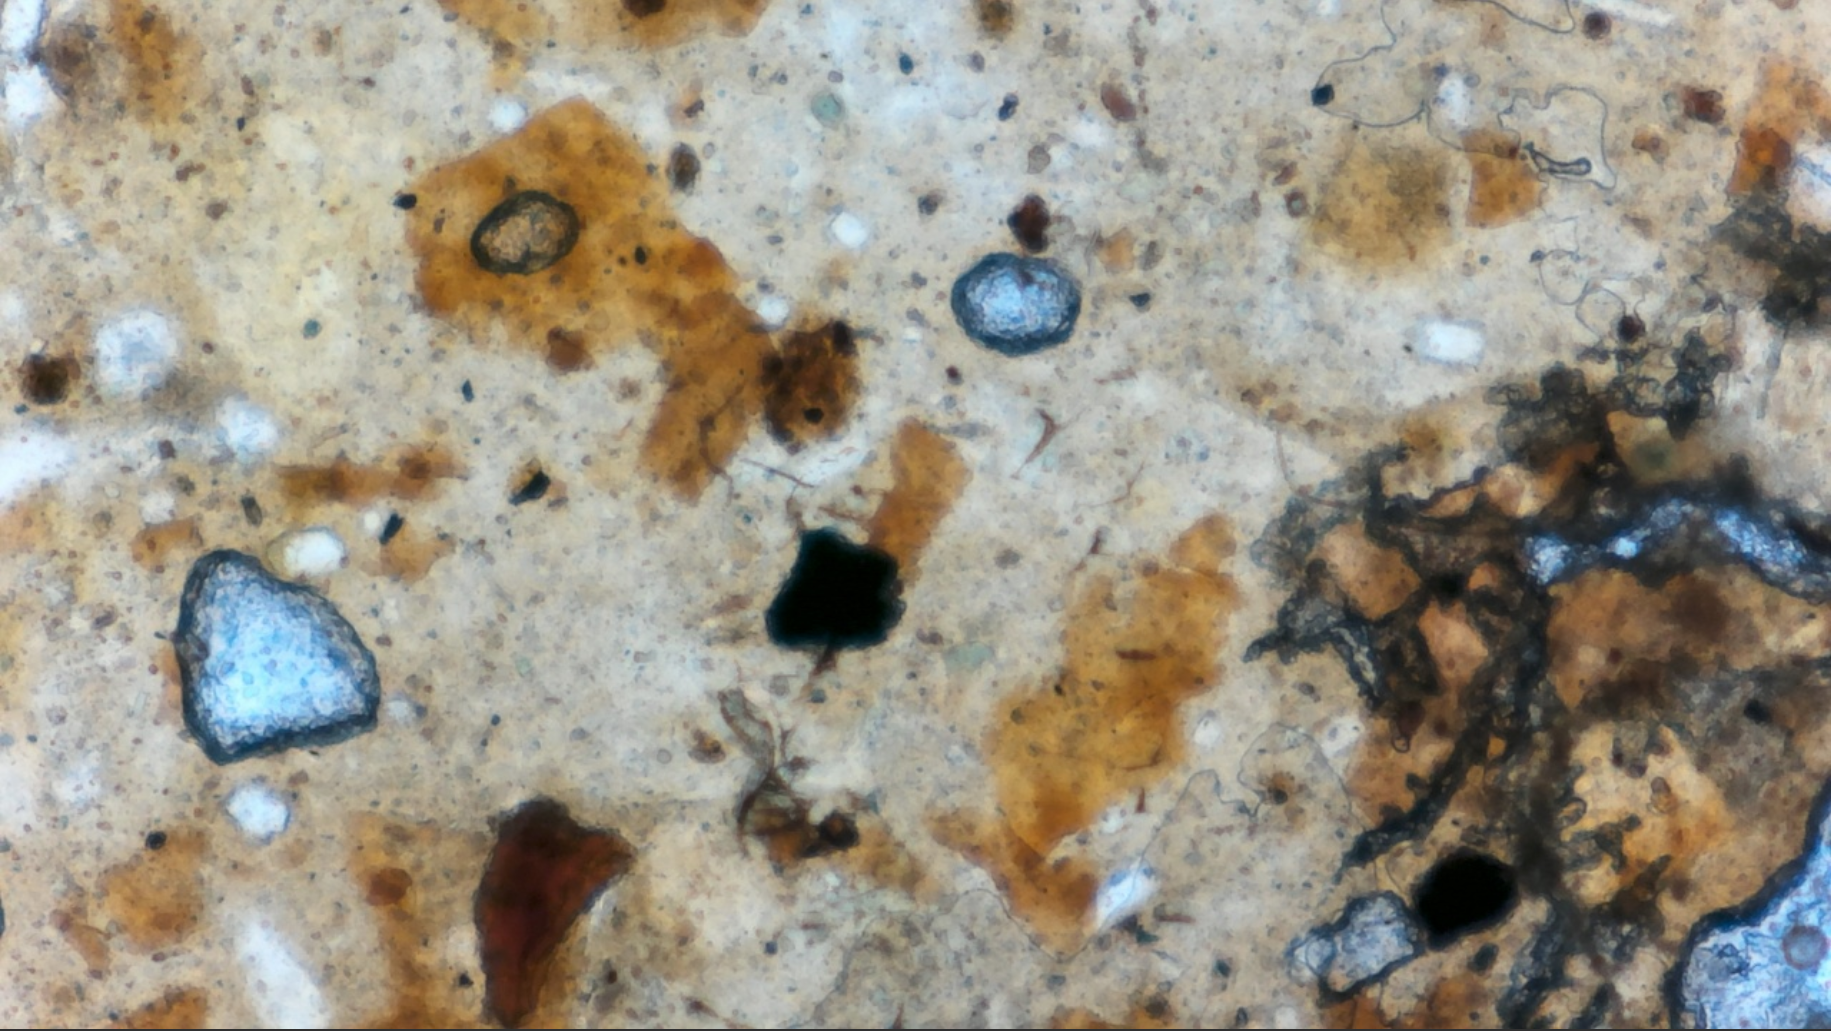
\includegraphics[width=\textwidth]{./img/subregion_focus.png}
        \caption{Image with subregions in focus.}
        \label{fig:focus}
    \end{subfigure}
    \hfill
    \begin{subfigure}[t]{0.3\textwidth}
        \centering
        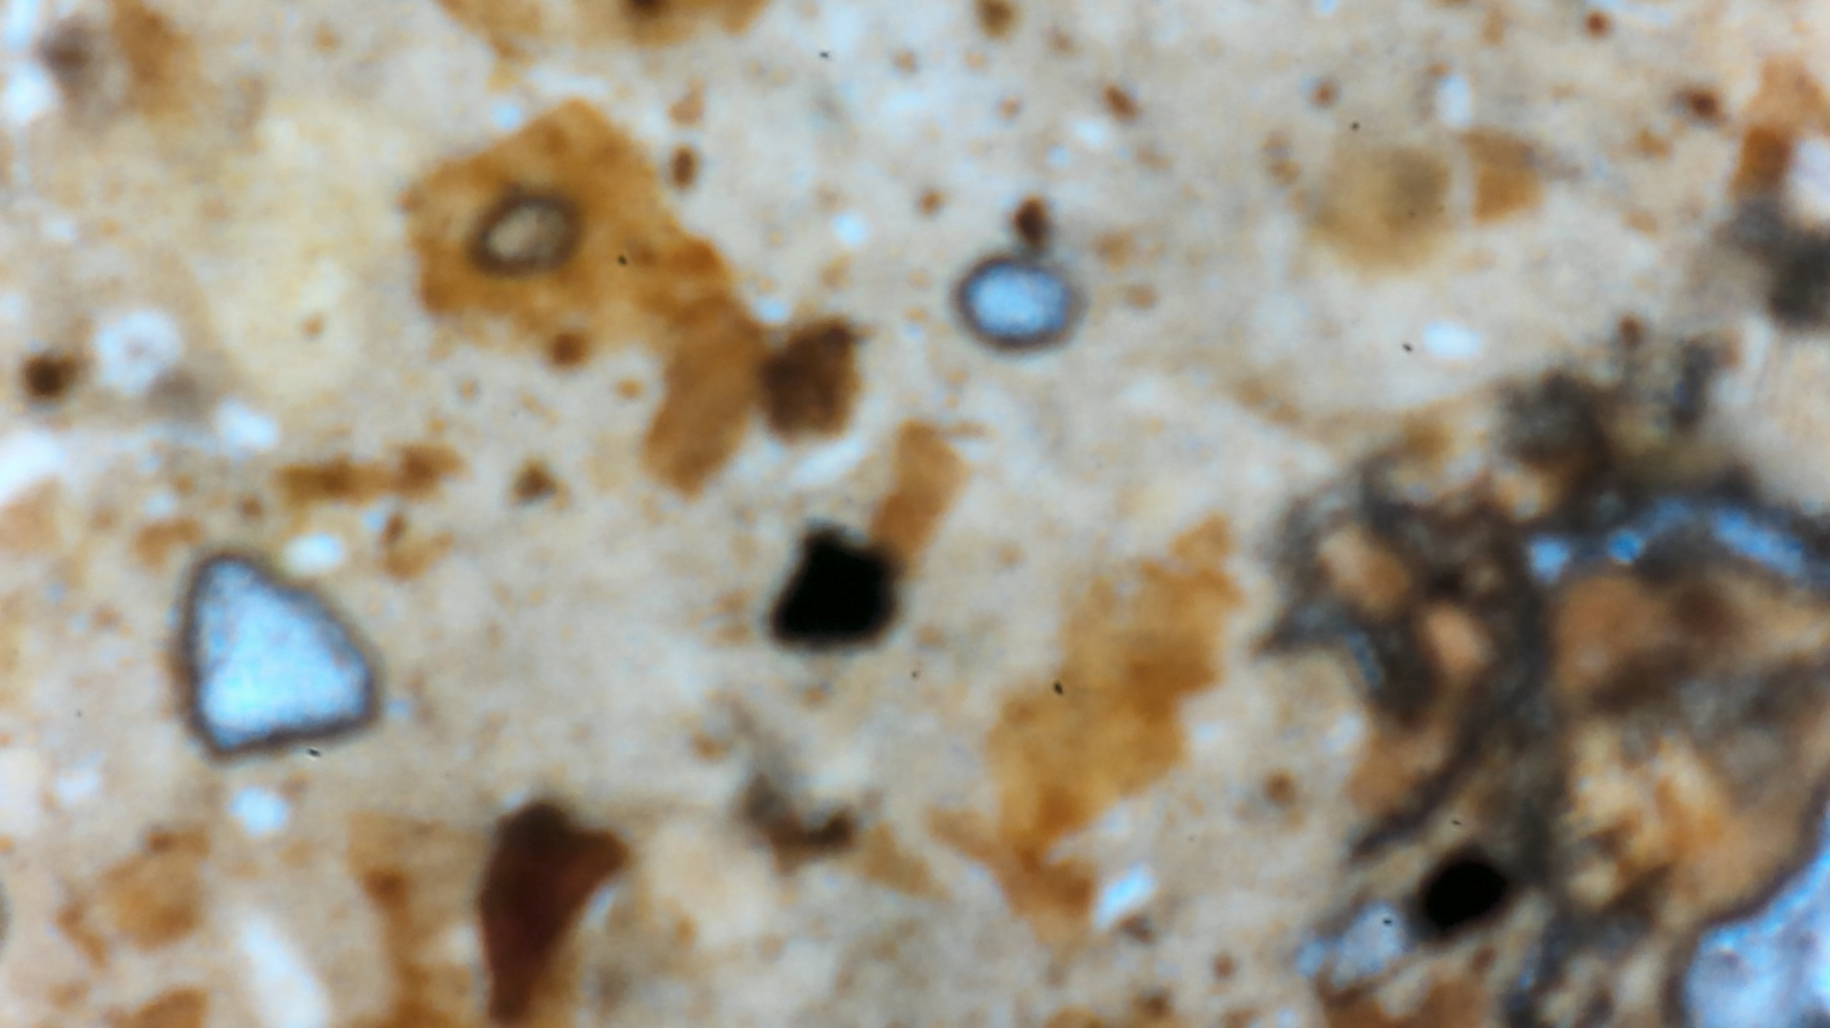
\includegraphics[width=\textwidth]{./img/out_of_focus_thither.png}
        \caption{Out-of-focus image with focal plane thither to sample.}
        \label{fig:focusThither}
    \end{subfigure}
    \caption{Three image samples.}
    \label{fig:focusComparison}
\end{figure}

\section{Description of the task}

\todo[inline]{Here you describe in more detail the contents of the project: what should be done and what moments are included. Specifically it should be described the interesting part of the problem, how this should be analysed and solved. Here there should be clarified that the project fulfils the requirements that the university has posed on a thesis project on this level.}

The z-stacking procedure has the drawback that it produces more data and time spent scanning each grid cell than other approaches and hence, an automatic procedure for determining the quality or distance to the focal plane is beneficial to reduce the costs. Due to the nature of the sample not all parts of the image are always in focus at the same time, therefore, the prediction should be made for subregions of the image. 


\section{Methods}

\todo[inline]{What systems, tools and methods should be used. Relevant literature (it is often a part of the work to find additional literature). How results should be evaluated and documented.}

Existing approaches have not been used on NTDs and most detect out of focus areas such as \emph{DeepFocus} \cite{senaras2018deepfocus}, \emph{ConvFocus} \cite{kohlberger2019wholeslide} and \emph{FocusLiteNN} \cite{wang2020focuslitenn}.

The dataset from Etteplan consists of non-annotated images which contain positional metadata. Therefore, a semi-supervised approach is used. The idea is to annotate a small subset of the dataset and to automatically label additional data. This can be either done by using an existing pre-trained and then fine-tuned model to find images that are in focus or by using other methods to detect in-focus images (see \citeauthor{yusun2005autofocusing} \cite{yusun2005autofocusing}). Images that are not in focus can then be annotated using a positional offset based on metadata of in-focus images on the same z-stack.

The results of the developed model are compared to an out of focus detection model. This can be done by converting the focus distance to a binary in-focus or out of focus label. Further, the focus distance estimation performance can be evaluated as is, but an appropriate metric has to be chosen.


\section{Relevant courses}

\begin{table}[H]
    \centering
    \begin{tabular}{|c|c|r|} 
        \hline
        Code & Name & ECTS \\
        \hline
        \texttt{1MD120} & Deep Learning for Image Analysis & 7.5 \\
        \texttt{1TD396} & Computer-Assisted Image Analysis I & 5.0\\
        \texttt{1DL073} & Natural Computation Methods for Machine Learning & 10.0 \\
        \texttt{1DL340} & Artificial Intelligence & 5.0\\
        \hline
    \end{tabular}
\end{table}

\section{Delimitations}

\todo[inline]{It is also important to specify what is not part of the project. This prevents that the thesis grows uncontrolled. You can add stuff that you can do if there is time left, also write down things that can be skipped if there are no time for them.}

The developed model will be based on a known, yet to be decided architecture and not a newly developed one.

\section{Time plan}

The time plan (see \autoref{fig:TimePlan:Gant}) is separated into two main parts. These are documentation and implementation. Initially literature research needs to be done and is considered to be a separate part but during the thesis new literature will need to be considered continuously. The initial literature research part coincides with parts of the documentation namely, background and methods as these parts are largely independent of the actual implementation. The implementation follows and is divided into four steps. First some data needs to be annotated, then based on these annotations additional data is automatically labelled. This is followed by a period of model development where at least one but potentially multiple models are developed and trained. Lastly, a full evaluation is done. During the phase of implementation material to all sections of the thesis document is added. This material is put into a coherent text in the following tasks. The implementation is expected to take from 10 to 11 weeks and the main parts of documentation 9 to 10 weeks.

\begin{figure}
    \begin{center}
        \begin{ganttchart}[y unit title=0.7cm,
            y unit chart=0.7cm,
            x unit=0.4cm,%0.25cm, 
            title height=1,
            bar height=0.6,
            group right shift=0,
            group top shift=.6,
            group height=.3,
            milestone label font=\footnotesize,
            title label font=\scriptsize,
            bar label font=\scriptsize,
            group label font=\small
            ]{3}{23}
            \gantttitle{2022}{21}\ganttnewline
            \gantttitlelist{3,...,23}{1}\ganttnewline
            \ganttgroup{Thesis}{3}{22}\ganttnewline
    
            \ganttgroup{Preparation}{3}{7}\ganttnewline
            \ganttbar{Literature Research}{3}{7}\ganttnewline

            \ganttgroup{Implementation}{8}{18}\ganttnewline
            \ganttbar{Dataset Annotation}{8}{10}\ganttnewline
            \ganttbar{Generating Annotations}{11}{12}\ganttnewline
            \ganttmilestone{Full Dataset}{12}\ganttnewline

            \ganttbar{Implementing Model}{13}{16}\ganttnewline
            \ganttmilestone{Trained Model}{16}\ganttnewline
            \ganttbar{Evaluate Model}{17}{18}\ganttnewline
            \ganttmilestone{Evaluation Scores}{18}\ganttnewline

            \ganttgroup{Documentation}{3}{22}\ganttnewline
            \ganttbar{Implementation Notes}{8}{17}\ganttnewline
            \ganttbar{Write Background}{4}{6}\ganttnewline
            \ganttbar{Write Methods}{7}{8}\ganttnewline
            \ganttbar{Write Results}{18}{18}\ganttnewline
            \ganttbar{Write Discussion}{18}{18}\ganttnewline
            \ganttbar{Write Introduction}{19}{19}\ganttnewline
            \ganttbar{Write Abstract}{20}{20}\ganttnewline
            \ganttmilestone{First Draft}{20}\ganttnewline
            \ganttbar{Finalize Thesis}{21}{21}\ganttnewline
            \ganttmilestone{Final Draft}{21}\ganttnewline
            \ganttbar{Proofread and Corrections}{22}{22}\ganttnewline
            \ganttmilestone{Finished Thesis}{22}\ganttnewline

            % into implementation
            \ganttlink{elem2}{elem4}
            \ganttlink{elem4}{elem5}
            \ganttlink{elem5}{elem6}

            
            \ganttlink{elem6}{elem7}
            \ganttlink{elem7}{elem8}
            \ganttlink{elem8}{elem9}
            \ganttlink{elem9}{elem10}

            % into documentation
            \ganttlink{elem10}{elem15}
            \ganttlink{elem15}{elem16}

                % into introduction
            \ganttlink{elem16}{elem17}
            \ganttlink[link mid=.65]{elem13}{elem17}
            \ganttlink{elem14}{elem17}

            \ganttlink{elem17}{elem18}
            \ganttlink{elem18}{elem19}
            \ganttlink{elem19}{elem20}
            \ganttlink{elem20}{elem21}
            \ganttlink{elem21}{elem22}
            \ganttlink{elem22}{elem23}

            \ganttvrule{}{7}
            %\ganttvrule{}{12}
            \ganttvrule{}{18}
            \ganttvrule{}{22}
        \end{ganttchart}
    \end{center}
    \caption{Gantt chart showing the time plan of the thesis by week.
    }
    \label{fig:TimePlan:Gant}
\end{figure}


\FloatBarrier 

\printbibliography[heading=bibintoc]
\end{document}